\documentclass{article}

\usepackage[utf8]{inputenc}
\usepackage[T1]{fontenc}
\usepackage{mathptmx}
\usepackage{csquotes}
\usepackage[margin=1in, bottom=1.25in, footskip=0.5in]{geometry}
\usepackage{parskip}
\usepackage{listings}
\usepackage{color}
\usepackage{lmodern}  % for bold teletype font
\usepackage{amsmath}  % for \hookrightarrow
\usepackage{xcolor}   % for \textcolor
\usepackage{pgfplots, pgfplotstable}
\usepackage{enumitem}
\usepackage[export]{adjustbox}
\usepackage{graphicx}
\usepackage{float}
\usepackage[sorting=none]{biblatex}
\usepackage{tikz}
\usepackage{subfig}

\pgfplotsset{compat=newest}
\setlength{\parindent}{0pt}
\setlist{leftmargin=1em}

\addbibresource{refs.bib}

\title{Visualising the Blockchain and Tracing Bitcoin Transactions}
\author{Matthew Consterdine \& Dennis Parchkov \& Altay Adademir}
\date{}

\begin{document}

\vspace*{-5em}

\begin{figure}[H]
  \centering
  \begin{tikzpicture}
  \draw (0, 0) node[inner sep=0] {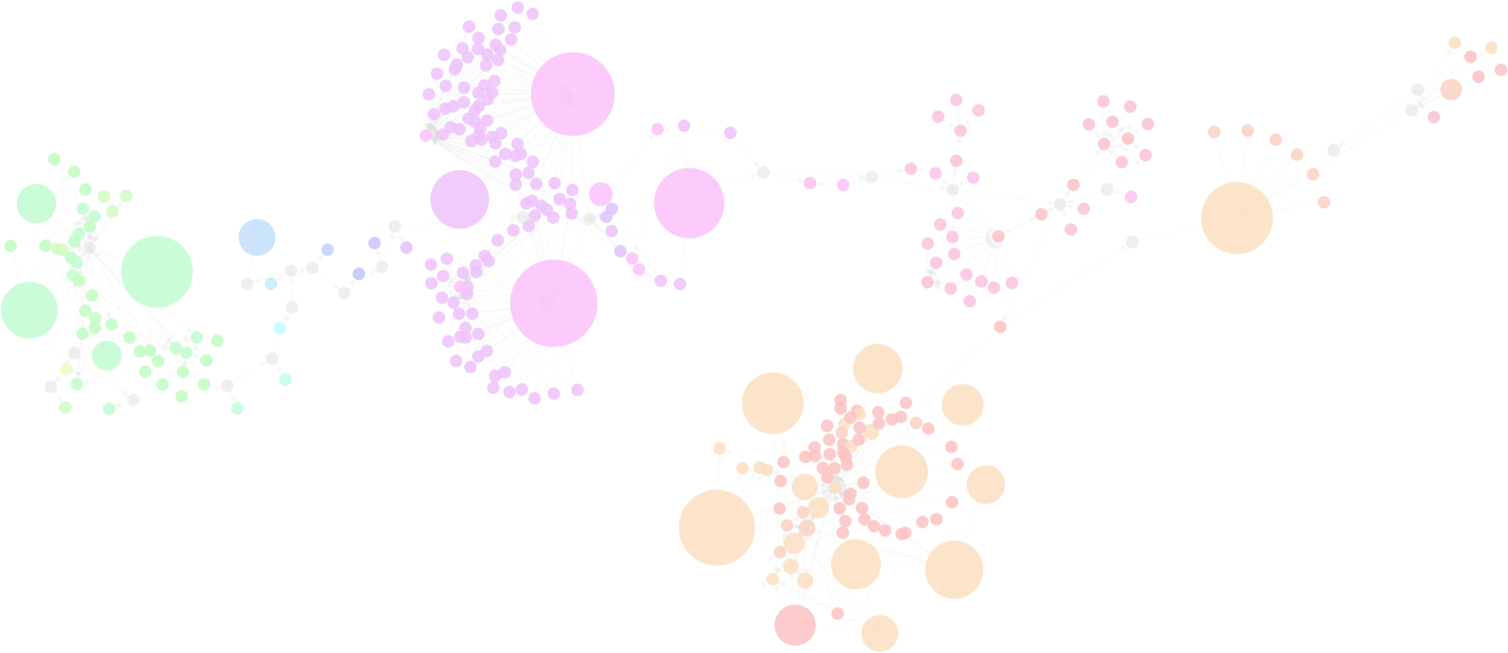
\includegraphics[max width=\textwidth]{images/distance-light.png}};
  \draw (0, 0.6) node {\huge Visualizing and Tracing Bitcoin Transactions};
  \draw (0, -0.6) node {\Large Matthew Consterdine \& Dennis Parchkov \& Altay Adademir};
%   \draw (4.3, -1.8) node {Figure 1};
  \end{tikzpicture}
  \label{fig:distancecolouringtitle}
\end{figure}
% \setcounter{figure}{1}
\vspace*{-3em}

\section*{Abstract}

This project demonstrates the ability to visualize, and trace transactions through the Bitcoin network, evaluating three different methods. Namely poison, haircut and First-In-First-Out (FIFO). 

To achieve this, a web application was created to first build up a network graph representing Bitcoin addresses as nodes, and transactions as directional edges. This allows the user to easily grasp the history of any given Bitcoin address, and then trace any transaction either up or down the graph.

\section{Background}

To trace Bitcoin transactions, a good knowledge of Bitcoin and how transactions work is needed. This section will explain this, then follow by exploring several different tracing techniques.

\subsection{Bitcoin Addresses}

Bitcoin addresses are generated from the public keys of the Elliptic Curve Digital Signature Algorithm (ECDSA), a form of public key cryptography. The keys are hashed multiple times with SHA256 and RIPEMD-160. The result is a set of twenty-six to thirty-five alphanumeric characters encoded using base58 in order to avoid visual ambiguity, specifically "O", "I","l","0" are never used \cite{antonopoulos2014mastering}. There are two widely used address formats:

\begin{itemize}
  \item P2PKH (Pay to public key hash): These addresses start with a 1 (i.e. 1AJbsFZ64EpEfS5UAjAfcUG8pH...) and are used when sending coins directly to an address. Currently the vast majority of transactions in the Bitcoin network use P2PKH.
  \item P2SH (Pay to script hash): These addresses start with a 3 (i.e. 3J98t1WpEZ73CNmQviecrnyiWrnqRh...) and allow for complex transaction unlocking processes such as requiring multiple keys or passwords. They also move the responsibility of providing the redeem conditions from the sender to receiver \cite{antonopoulos2014mastering}.
\end{itemize}

\subsection{Bitcoin transactions}

To understand transactions in Bitcoin, the coin analogy is used. Suppose a user has an account that has received three separate transactions of (1 BTC, 3 BTC and 5 BTC). The account balance would be 8 BTC but only contain three coins. A coin can thus be defined as an incoming transaction regardless of the value. Now sending someone 4 BTC can be achieved in a number of different ways \cite{antonopoulos2014mastering}:

\begin{itemize}
  \item Merge the 1 BTC and 3 BTC coins to produce a 4 BTC coin for the recipient,
  \item Take the 5 BTC coin and split it in to two coins (1 BTC and 4 BTC) sending 4 BTC to the recipient and sending 1 BTC back to the original account (change).
\end{itemize}

With Bitcoin it is impossible to spend a fraction of a coin and keep the rest. Any remainder must be explicitly returned to the original address. This is different to traditional banking where account balances may as well be an integer in a database. As such, a raw Bitcoin transaction has the following components:

\begin{itemize}
  \item Inputs: Unspent outputs of previous transaction and the first half of the script used to unlock the transaction (ScriptSig)
  \item Outputs: Where the coins are going to, and change followed by the second half of the script (ScriptPubKey) used for locking the coins. Inputs that are not redeemed in the outputs are considered transaction fees.
\end{itemize}

Bitcoin transaction verification system is based on  a scripting language that pushes the scripts (ScriptSig and ScriptPubKey) on to a stack. If by the end of the process the stack is empty with no errors, then the output unlock script successfully managed to redeem the outputs \cite{antonopoulos2014mastering}.

Verification process can be a very simple process (such as providing a private key) or can be complex such as require multiple keys or provide a password \cite{antonopoulos2014mastering}.

\subsection{Tracing Methods}

\begin{figure}[H]
  \centering
  \subfloat[Poison]{{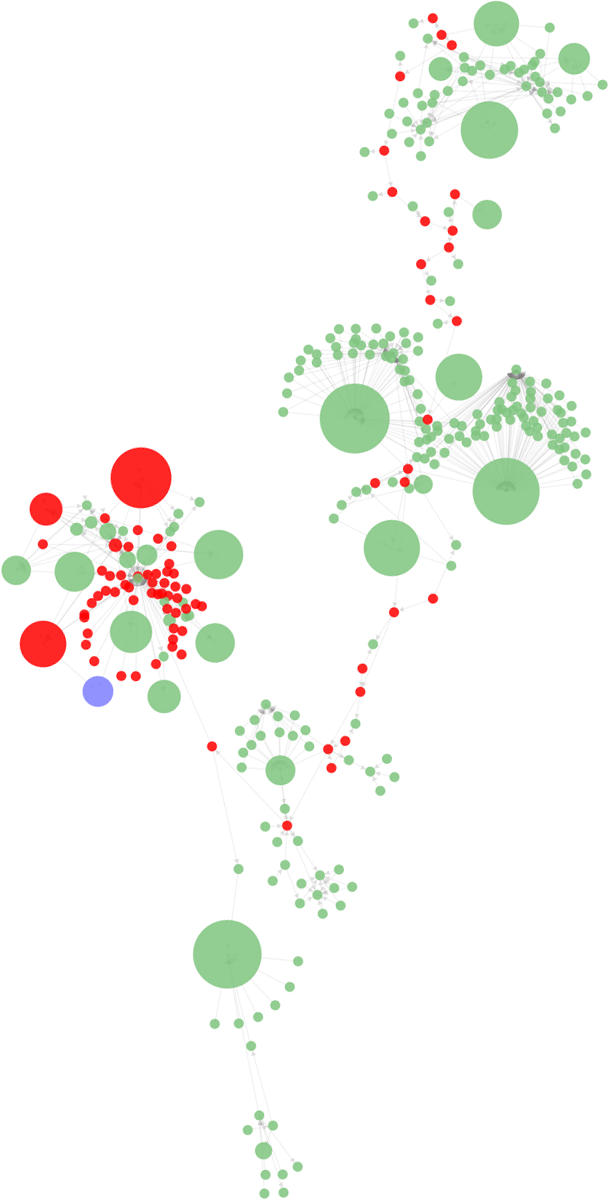
\includegraphics[width=4cm]{images/poison.png}}}
  \qquad
  \subfloat[Haircut]{{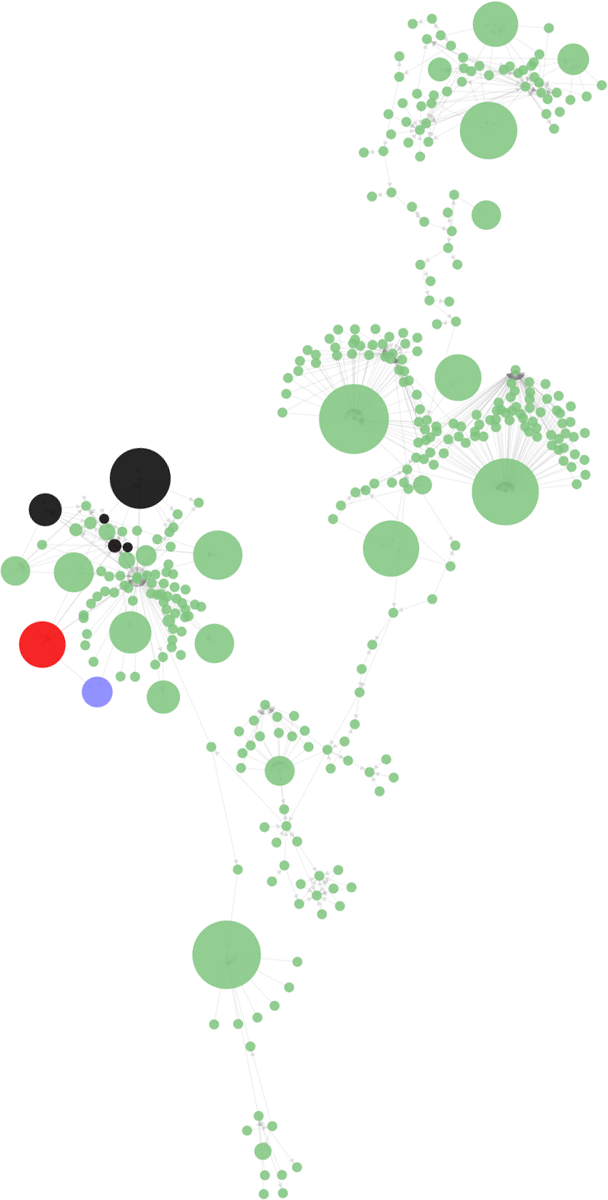
\includegraphics[width=4cm]{images/haircut.png}}}
  \qquad
  \subfloat[FIFO]{{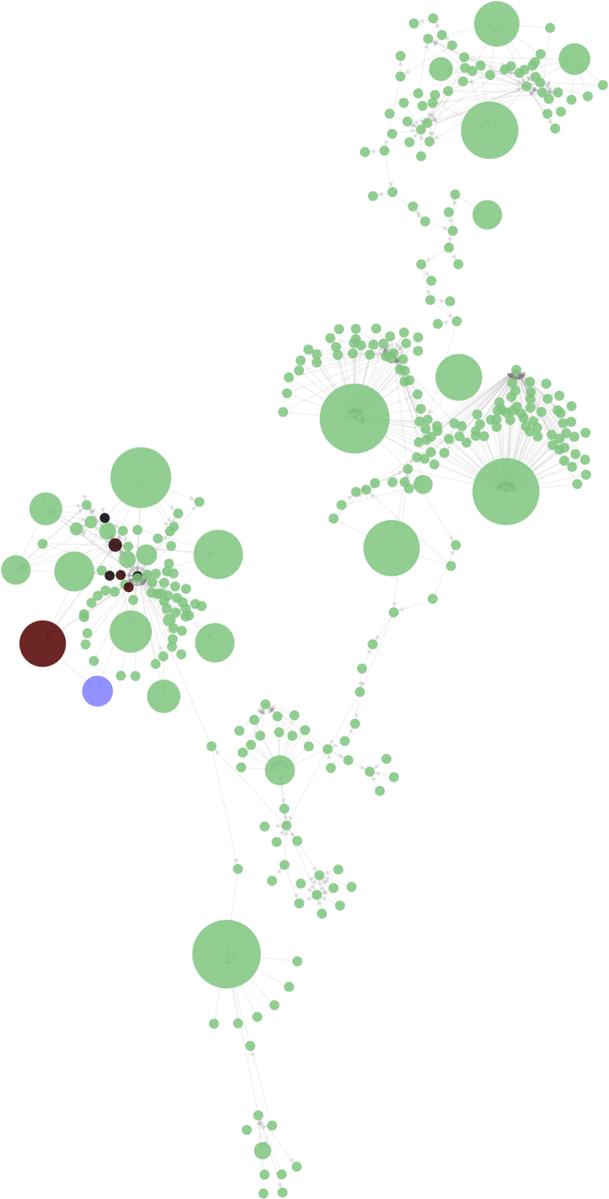
\includegraphics[width=4cm]{images/fifo.png}}}
  \caption{Comparing Different Tracing Methods}
  \label{fig:tracingmethods}
\end{figure}

The following examples all refer to the following situation: Given 3 addresses A (10 BTC), B (5 BTC) and C (20 BTC), trace the transaction of 10 BTC from address A. A transfers 10 BTC to B and B transfers 5 BTC to C. The end result is A (0 BTC), B (10 BTC) and C (25 BTC). Transactions fees are ignored.

\subsubsection{Poison}

Taint all BTC in transfers and address\cite{stolenbtc}. With the scenario listed above, 100\% of the coins in B would be tainted and 100\% in C would be tainted. If B or C transfers money to any address, those addresses would also be 100\% tainted no matter the amount. This does not provide a scalable way of tracing as with a huge amount to transfers would result in a huge amount of addresses possibly creating confusion.

\subsubsection{Haircut}

Taint everything proportionally based upon how much comes from the original transaction. With the scenario above, all B BTC would be 50\% tainted BTC and all C coins are 20\% tainted. By sending coins to multiple accounts, the taint on the coins becomes diluted and would eventually disappear\cite{stolenbtc}. Diluting coins is an easy mechanism for criminals to do as it is pretty similar to how traditional money laundering schemes operate.  
    
\subsubsection{FIFO}

Queue based approach, first in first out. All the coins transfered to B are tainted. As B already has 5 clean BTC, the 5 BTC transfered to C would be clean, thus B would have no tainted coins. The next set of transactions that B performs would result in those coins being tainted (add to 10 BTC). If B receives clean coins these would be placed after the tainted ones \cite{stolenbtc}.

\subsection{Anonymity}

Bitcoin is not anonymous, Bitcoin is pseudo-anonymous. While user identities are concealed, all transactions are publically listed in the blockchain and it is likely that a nation state could tie Bitcoin addresses to identities. Additionally, many people choose to publically disclose their addresses. This is understandable given that this is required to pay for goods or services.

\section{Implementation}

After researching and judging whether or not this project was possible, the team set out to create it.

\subsection{Blockchain API}

As setting up a full node with the entire blockchain would require an excessive amount of storage (approximately 150 GB as of 2018), the team decided to use a third-party API, blockchain.info, for the purpose of retrieving information on the Bitcoin blockchain \cite{blockchain_2018_open}.

However by using such a service, ease of use is traded for security. The API could easily and undetectably falsify results, but given the prominence of the API in question and it's many fund-raising rounds, this is deemed unlikely. Regardless, it would not be entirely wise to trust the data entirely.

Additionally, blockchain.info provides and verifies a Bitcoin address tagging service. The data of which is used to provide the user with user friendly names. However, the dataset is small.

\subsection{Graphing the Blockchain}

\begin{figure}[H]
  \centering
  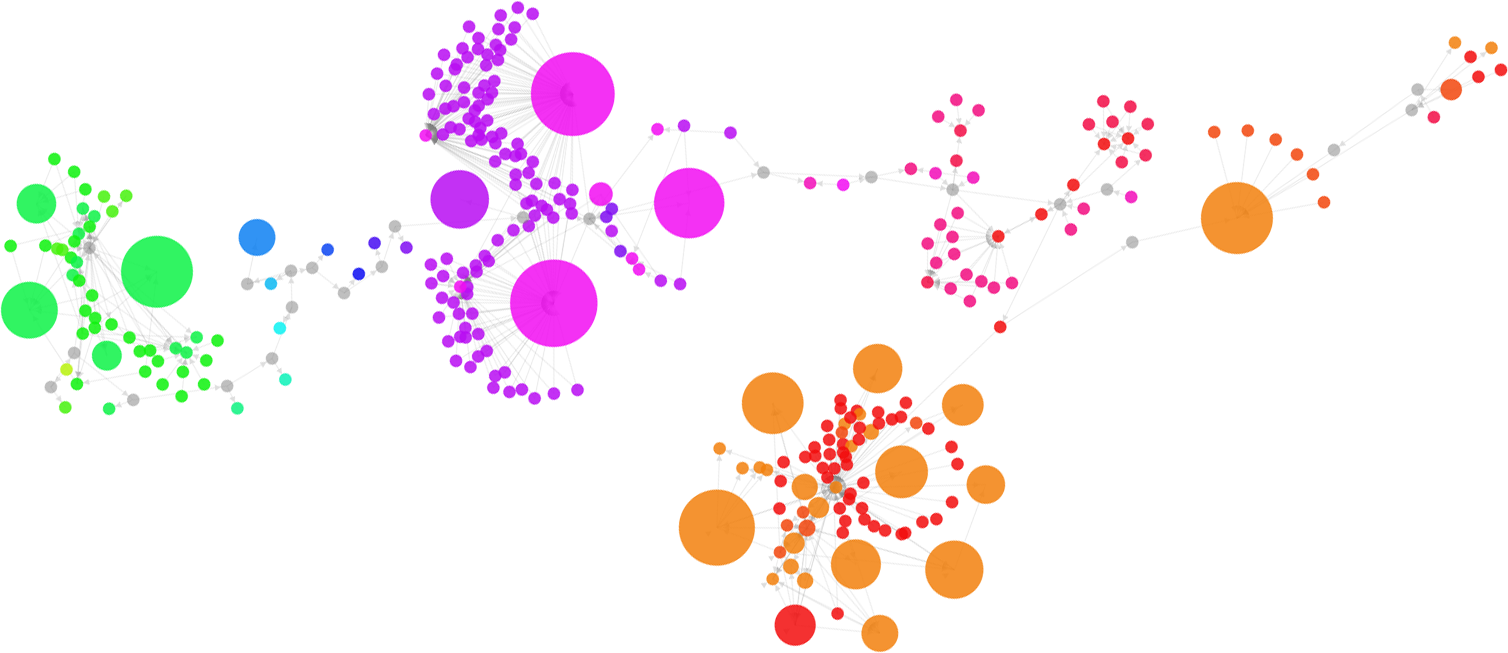
\includegraphics[width=0.6\textwidth]{images/distance.png}
  \caption{Distance Dependent Colouring}
  \label{fig:distancecolouring}
\end{figure}

To represent the Bitcoin blockchain, the team decided to flatten time turning the Merkle Tree into a networked graph. By doing so, it is trivial to represent the many transactions between different addresses, revealing structure and complex interconnections that would be invisible otherwise.

After evaluating the different options the team decided to use D3.js, a popular JavaScript framework for creating 'Data-Driven Documents' and visualizations \cite{d3js}. Specifically, the force layout option was used.

In the networked graph above, the distance away from the original address is used to shift the hue, producing pretty visuals. For other uses, a monochromatic colour scheme is available.

To calculate the size of a given node, the balance of the address represented is either explicitly loaded by the user, or is estimated. This is done by examining all of the known incoming and outgoing transactions to calculate the final balance. This is not that accurate, but is the best approach. It provides good visual feedback, pointing the user in the right direction.

\subsection{User Experience}

\begin{figure}[H]
  \centering
  \subfloat[Application]{{\fbox{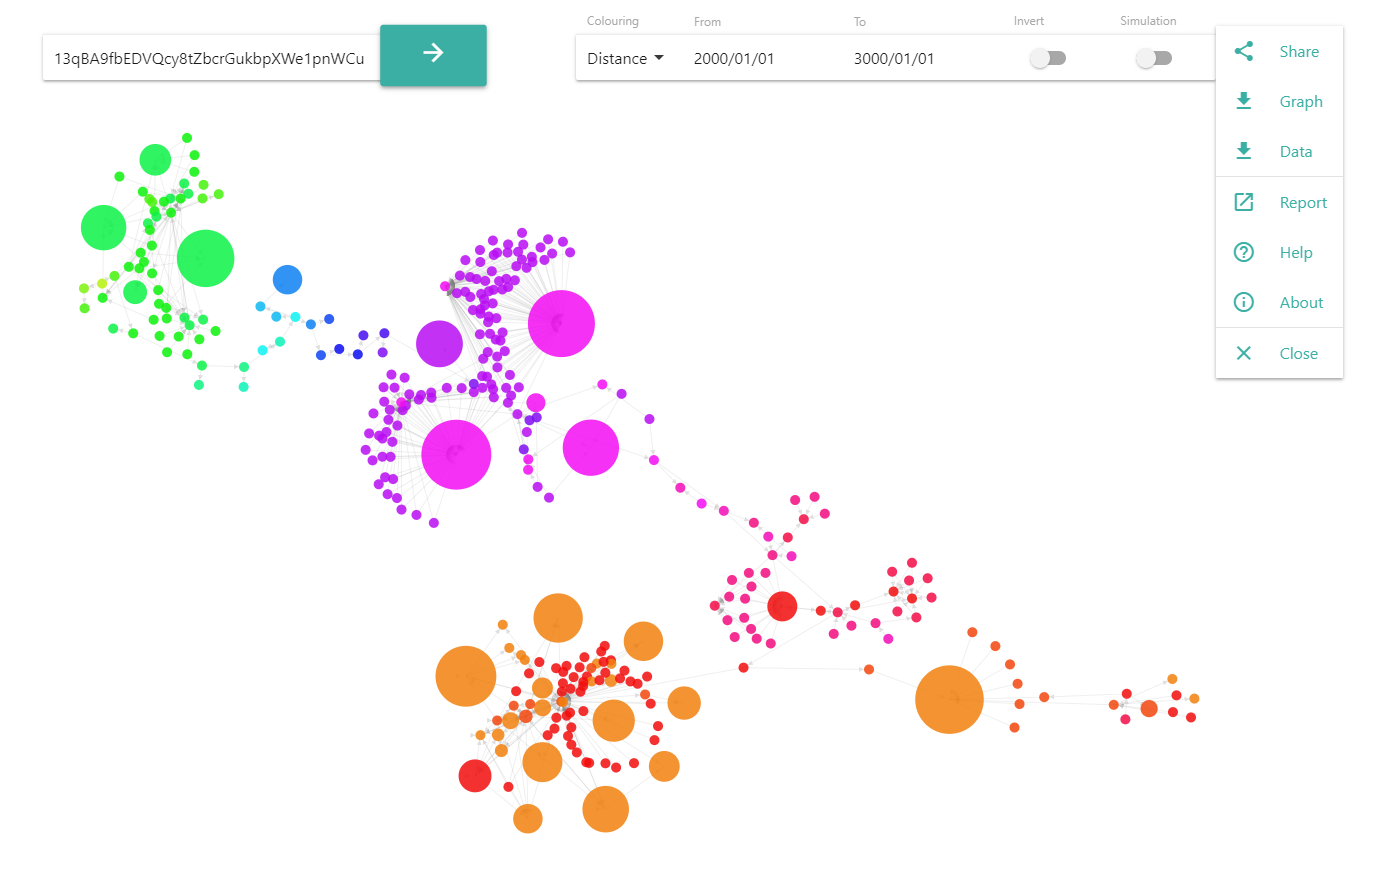
\includegraphics[width=10cm]{images/application.png}}}}
  \qquad
  \subfloat[Tooltip]{{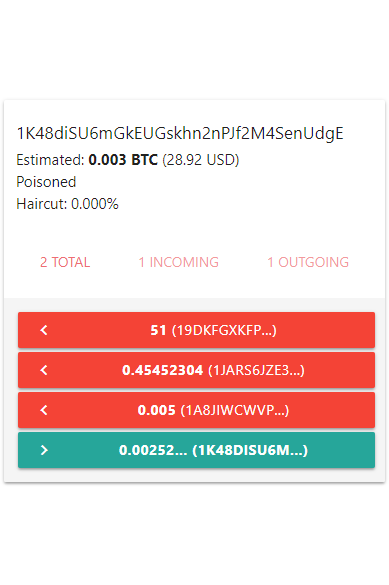
\includegraphics[width=4cm]{images/tooltip-padded.png}\vspace*{1.5cm}}}
  \caption{User Experience}
  \label{fig:userexperience}
\end{figure}

To create the look and feel of the application, the MaterializeCSS framework was used. It is a popular CSS framework that follows Google's Material Design standard \cite{materializeabout} and provides a number of useful components to build from. In the right hand dropdown menu, the user can export the graph, read the report, or learn.

By clicking on a node in the graph, the application will automatically load that address and it's associated transactions, adding it to the graph. By hovering over a node in the graph, the tool-tip on the right will appear. It displays a number of useful statistics about the address, and gives the user the option to trace transactions by clicking on any of the colourful buttons.

If the user wishes, they can constrain the date range to narrow down which transactions are loaded. The simulation can be paused, and the nodes can be rearranged by dragging and dropping.

\section{Limitations and Future Work}

\subsection{Modeling Transaction Fees}

Currently transaction fees are ignored, potentially leading to small errors in tracing. For greater precision, time could be taken to model transaction fees. New interface elements would be needed.

\subsection{Live Updates}

Blockchain.info web sockets can be used as a live data feed for the Bitcoin network. Live data could be automatically added onto existing nodes to show transactions in real-time.

\section{Conclusion}

The team successfully created an easy to grasp, network graph visualization of the Bitcoin blockchain. It helps to reveal the many messy interconnections by structuring the results using a D3.js force layout. It is also visually appealing to look at.

Transactions can be traced up or down the blockchain with the press of a button. Different techniques were used including Poison, Haircut, and FIFO. Poison is useful if basic and broad, haircut allows the user to see how Bitcoins are evenly distributed, and FIFO allows for significantly refined tracing. Each technique is useful in it's own way, but ultimately only FIFO traces Bitcoins in an actionable manner.

\section*{References}

\nocite{*}
\printbibliography[heading=none]

\end{document}
